\documentclass[11pt]{article}
\usepackage[a4paper,margin=1in]{geometry}
\usepackage{amsmath,amssymb,amsthm,mathtools}
\usepackage{graphicx,booktabs,array,enumitem,hyperref,microtype}
\setlength{\emergencystretch}{2em}
\hypersetup{colorlinks=true,linkcolor=black,citecolor=blue!50!black,urlcolor=blue!50!black}
\newtheorem{definition}{Definition}
\newtheorem{proposition}{Proposition}
\newtheorem{corollary}{Corollary}
\newcommand{\Tr}{\operatorname{Tr}}
\newcommand{\GMVP}{\Gamma_{\mathrm{MVP}}}

\title{\textbf{Physical Parent Selection for a Common Tau Completion}\\
\large Tau Core Foundation Paper IV --- Preparation Manuscript}
\author{Jozsef Olcsak\\\small Independent researcher}
\date{Preparation v0.1 --- 2026}

\begin{document}
\maketitle

\begin{abstract}
The first three Tau Core foundation manuscripts leave one shared physical
arrow open: whether one physical base--seed source selects and occupies the
common completion used in their conditional architecture, finite source and
record-transport results.  We isolate that arrow without using terminal fit
quality as a selector.  On a finite retained body/certificate fiber we prove
an exact nonselection theorem: a joint comparison potential and a split
potential satisfy the same current pure-axis source laws and the same occupied
seed support while differing in their mixed Hessian.  Universal-seed
occupation therefore does not select the joint law.  We then prove a minimal
positive theorem.  If the certificate is physically typed as the
Legendre-conjugate response of the stabilized body under one source-frozen
strictly convex parent potential and complete mediation forbids a bypass, the
joint Fenchel--Young law is unique on the retained support and introduces no
independent gain.  A complete faithful source signature would subsequently
select one completion class as the unique zero of a positive source defect.
The manuscript is a preparation packet: the physical parent has not yet been
shown to select the certificate semantics, the complete signature, or
\(\GMVP\). Nature-level selection remains open.
\end{abstract}

\tableofcontents
\clearpage

\section{Question and series interface}

The sole question owned by this paper is
\begin{equation}
 B_\tau^{\mathrm{phys}}+s_U\Longrightarrow\GMVP\;?
 \label{eq:selection-question}
\end{equation}
Here \(s_U\) is one occupied universal morphology seed and
\(B_\tau^{\mathrm{phys}}\) is an enriched response-capable base.  The desired
conclusion is not merely existence of a completion but physical selection of
the same once-counted source packet, occupied support and common unit used by
the downstream constructions.

The interface is forward-only:
\begin{equation}
 \text{architecture}\longrightarrow
 \text{source selection}\longrightarrow
 \text{record transport}\longrightarrow
 \text{terminal laws}.
\end{equation}
A terminal agreement or recovery theorem cannot be read backward as a source
selection proof.

\begin{figure}[t]
 \centering
 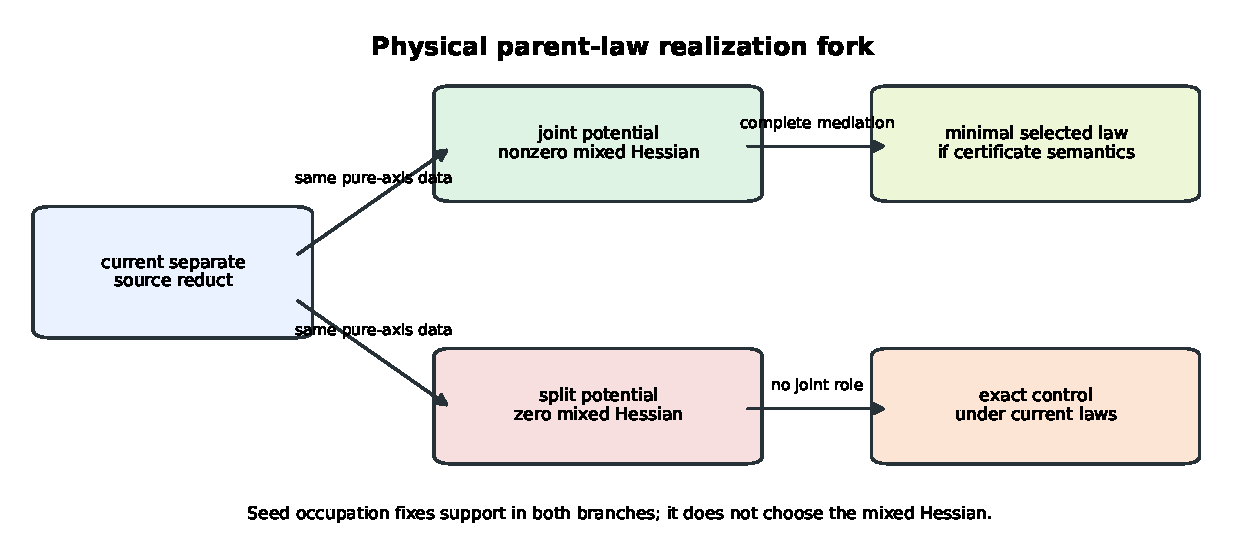
\includegraphics[width=.95\linewidth]{figures/fig_parent_selection_fork.pdf}
 \caption{The finite parent-selection fork.  Current separate source data admit
 both branches.  Certificate semantics plus complete mediation select the
 upper branch conditionally.}
 \label{fig:selection-fork}
\end{figure}

\section{Claim boundary}

This preparation manuscript proves a finite countermodel and conditional
representation results.  It does not prove that Nature realizes the Tau
ontology, that the physical parent selects \(\GMVP\), or that time, quantum
theory, gravity, matter or gauge physics have been derived from the selected
source.  Strict convexity selects a stationary response after a potential is
given; it does not select the potential family.  Seed occupation selects an
occupied support; it does not create a missing mixed source relation.

\section{Finite body--certificate reduct}

Let \(V_\chi\) be the retained real source fiber at occupancy
\(\chi\in\{0,1\}\), and let \(P_\chi\) be its orthogonal support projector.
The coordinate \(y\in V_\chi\) represents a typed certificate and
\(z\in V_\chi\) the corresponding stabilized-body descriptor.  Fix one
positive inherited unit \(\mu_0\).

The current separate source reduct fixes positivity, smoothness, covariance,
the two pure-axis Hessians and the occupancy projector:
\begin{equation}
 H_{yy}=H_{zz}=\mu_0P_\chi.
 \label{eq:pure-axis-data}
\end{equation}
It does not independently fix \(H_{yz}\).

\section{Exact nonselection theorem}

Define two source-frozen actions
\begin{align}
 \mathcal A_{\rm joint}(y,z)
 &=\frac{\mu_0}{2}\lVert P_\chi(y-z)\rVert^2,\label{eq:joint}\\
 \mathcal A_{\rm split}(y,z)
 &=\frac{\mu_0}{2}\bigl(\lVert P_\chi y\rVert^2
 +\lVert P_\chi z\rVert^2\bigr).\label{eq:split}
\end{align}

\begin{proposition}[Current-reduct nonselection]
The actions in Eqs.~\eqref{eq:joint}--\eqref{eq:split} satisfy the same
positive pure-axis data, covariance and occupied projector, but are inequivalent
as joint source laws.  Therefore the current separate source reduct does not
select the joint potential.
\end{proposition}

\begin{proof}
Both actions are nonnegative, twice differentiable and depend only on the
retained support.  Direct differentiation gives Eq.~\eqref{eq:pure-axis-data}
for both.  Their mixed Hessians are
\begin{equation}
 H_{yz}^{\rm joint}=-\mu_0P_\chi,
 \qquad H_{yz}^{\rm split}=0.
\end{equation}
No support-preserving change of variables that retains the typed \(y\) and
\(z\) roles maps a zero mixed block to the nonzero inherited block.  They are
therefore distinct completions of the same declared reduct.
\end{proof}

\begin{corollary}[Seed-support ceiling]
Selecting \(P_1\) by one occupied universal seed does not distinguish the two
actions.
\end{corollary}

\begin{proof}
Both actions restrict to the same \(P_1\).  Occupation changes the domain but
does not supply the absent mixed derivative.
\end{proof}

\section{Conditional minimal positive theorem}

Let \(\Phi_\chi:V_\chi\to\mathbb R\) be a source-frozen \(C^2\), strictly
convex potential.  Its Fenchel--Young defect is
\begin{equation}
 \mathcal D_{\Phi_\chi}(y,z)=
 \Phi_\chi(y)+\Phi_\chi^*(D\Phi_\chi(z))
 -\langle y,D\Phi_\chi(z)\rangle.
 \label{eq:fy}
\end{equation}

\begin{definition}[Physical certificate semantics]
The retained certificate is physical when it is the Legendre-conjugate
response to the body descriptor under the same parent potential, and complete
mediation excludes a second independent certificate/body bypass on the same
typed support.
\end{definition}

\begin{proposition}[Minimal joint completion]
Under physical certificate semantics, Eq.~\eqref{eq:fy} has a unique zero at
\(y=z\) in the source-normalized chart.  For
\(\Phi_\chi(u)=\mu_0\lVert P_\chi u\rVert^2/2\), it reduces exactly to
Eq.~\eqref{eq:joint}.  No independent tether gain is required.
\end{proposition}

\begin{proof}
Fenchel--Young inequality gives \(\mathcal D_{\Phi_\chi}\ge0\), with equality
when \(D\Phi_\chi(y)=D\Phi_\chi(z)\).  Strict convexity makes the gradient
injective on the retained support, hence equality holds exactly at \(y=z\).
Substitution of the quadratic potential yields Eq.~\eqref{eq:joint}.  Its scale
is the inherited \(\mu_0\); another gain would duplicate the declared source
unit.
\end{proof}

This proposition is a uniqueness theorem inside a typed physical-certificate
completion.  It is not a derivation that the physical parent chooses that
semantics.

\section{Complete source-signature selector}

Let \(\mathfrak C\) be the finite set or moduli space of admissible completion
classes after declared source isometries.  Suppose the physical source supplies
an endpoint-blind signature \(\Sigma_s\) and a once-counted signature map
\(\Phi_s:\mathfrak C\to\mathcal V_s\).  Define
\begin{equation}
 \mathcal D_s(C)=\lVert\Phi_s(C)-\Sigma_s\rVert^2.
 \label{eq:source-defect}
\end{equation}

\begin{proposition}[Conditional source selection]
If \(\Phi_s\) is faithful on completion classes modulo declared typed source
isometry and \(\Sigma_s\) lies in its image, then
\(\mathcal D_s\) has exactly one zero completion class.
\end{proposition}

\begin{proof}
Existence follows from \(\Sigma_s\in\operatorname{im}\Phi_s\).  If two classes
have zero defect, their images are equal to \(\Sigma_s\); faithfulness makes
the classes equal modulo the declared isometry.
\end{proof}

The missing physics is now finite but substantial: construct and physically
occupy one signature containing the body response, joint incidence, common
unit, record occurrence and all distinguished roles needed by the claimed
completion.  A list of compatible terminal marginals is not such a signature.

\section{Proof ledger}

\begin{center}\small
\begin{tabular}{p{.48\linewidth}p{.18\linewidth}p{.24\linewidth}}
\toprule
Statement & Status & Consequence\\
\midrule
Joint/split counterpair shares current separate reduct & proved & current laws do not select\\
Seed occupation fixes support but not mixed Hessian & proved & seed alone is insufficient\\
Certificate semantics selects the joint convex law & conditional theorem & unique minimal candidate\\
Faithful complete signature has one zero class & conditional theorem & finite selection target\\
Physical parent supplies certificate semantics & open & Paper IV blocker\\
Physical parent supplies and occupies full signature & open & nature-selection blocker\\
Full signature equals the complete \(\GMVP\) packet & open & interface to Papers I--III\\
\bottomrule
\end{tabular}
\end{center}

\section{Finite work program}

The preparation phase has four bounded tasks:
\begin{enumerate}[label=(W\arabic*)]
 \item Freeze the exact completion signature required by \(\GMVP\), removing
 duplicates already generated by one source relation.
 \item Determine whether physical certificate semantics follows from an
 independently required parent role, rather than being chosen to obtain the
 joint action.
 \item Construct the corresponding once-counted microscopic ledger and audit
 all cross derivatives for double counting and quotient descent.
 \item Produce either a source theorem selecting the occupied class or a finite
 same-reduct countermodel proving that further nature-level selection is
 impossible without genuinely new typed source information.
\end{enumerate}

No fifth task may be added at the same level.  Failure of W2 or W3 demotes the
current positive candidate and fixes the no-go result as the principal Paper
IV conclusion.

\section{What is not proved}

Nature-level selection remains open.  In particular, this manuscript does not
derive the universal seed from a prior temporal process, prove that the
physical base realizes the adopted convex/Frobenius packet, identify a
laboratory carrier, determine SI constants, or recover the full Standard
Model.  It also does not promote a successful downstream terminal fit into
evidence for Eq.~\eqref{eq:selection-question}.

\section{Conclusion}

The physical parent-selection problem is neither an unlimited search nor a
solved theorem.  Current source laws admit an exact joint/split counterpair,
so seed occupation and separate positive Hessians are insufficient.  A typed
physical-certificate semantics selects one minimal joint convex law, and a
faithful complete source signature would select one completion class.  The
remaining Paper IV task is to derive or falsify physical ownership of those
two inputs from one base--seed parent ledger.

\end{document}
